\documentclass[a4paper]{article}
\usepackage[margin=2cm]{geometry}

\usepackage{animate}
\usepackage{graphicx}
\usepackage{fontspec}
\usepackage[catalan]{babel}
\usepackage{hyperref}
\usepackage{float}

\hypersetup{
	colorlinks = true,
	linkcolor = black,
	urlcolor = blue,
}

\setlength{\parindent}{0pt}
\setlength{\parskip}{0.2cm}

\begin{document}
\begin{titlepage}
	\centering
	\vspace{1cm}
	
\includegraphics[width=0.25\textwidth]{images/etseib}
	\par\vspace{1cm}
	\textsc{ \LARGE Escola Tècnica Superior d'Enginyeria \\[1em] 
		Industrial de Barcelona}
	\par\vspace{2cm}
	\textbf{\Huge Tècniques Estadístiques per la Qualitat}
	\par\vspace{2cm}
	{\LARGE Informe pràctiques}
	\vfill
	\begin{flushright}
		\large
		Marc Asenjo i Ponce de León \par
		Joan Marcè i Igual \par
		Iñigo Moreno i Caireta \par
		Esteve Tarragó Sanchís \par
	\end{flushright}
\end{titlepage}

\tableofcontents
\pagebreak

\section{Introducció}
En aquest treball s'han usat les tècniques de disseny d'experiments per poder veure el funcionament d'un sistema. Per tal de poder tenir una motivació més alta, s'ha contactat amb l'empresa \emph{Proteïn S.A.} de manera que el cas presentat fos un real. 

\subsection{Sistema a estudiar}
L'activitat principal de \emph{Proteïn S.A.} és fabricar  \emph{\href{https://es.wikipedia.org/wiki/Col\%C3\%A1geno_hidrolizado}{co\l.lagen hidrolitzat}} a partir de l'ós de porc. A part un subproducte que genera és el \emph{\href{https://es.wikipedia.org/wiki/Fosfato_tric\%C3\%A1lcico}{Fosfat Tricàlcic}} ($Ca_3 (PO_4)_2$) o també conegut com \emph{apatita}. La característica principal de l'apatita és que els compradors la volen amb un \% en massa superior al 15\%. Si aquesta condició no es pot garantir els clients reclamaran indemnitzacions o aniran a comprar a la competència.

Per poder saber quins factors s'han de controlar cal entendre primer com funciona la part del procés d'on s'obté l'apatita, veure \autoref{fig:esquema}. Inicialment el producte arriba del procés anterior i conté co\l.lagen i apatita en suspensió en aigua (línia blava al P\&D). Així doncs, s'ha de separar l'apatita de l'aigua, el problema és que precipita molt fàcilment i s'ha de forçar que es mantingui en suspensió. Per tant, hi ha una sèrie d'elements que asseguren que això sigui així; al dipòsit on va a parar (C-03) hi ha un parell de barrejadors i una bomba de recirculació (P-C32). 

\begin{figure}[H]
	\centering
	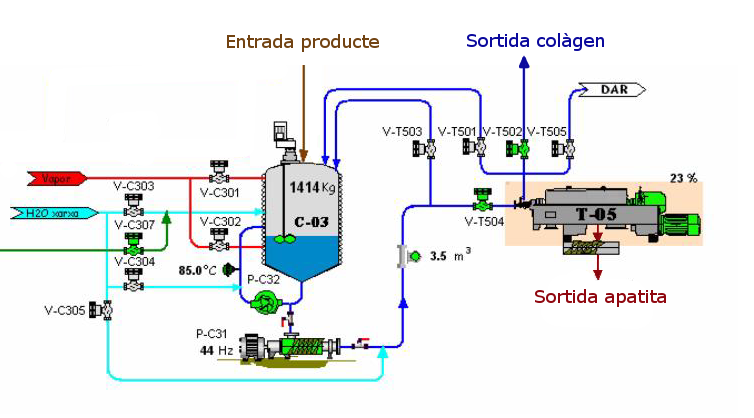
\includegraphics[width=0.8\textwidth]{images/esquema}
	\caption{Esquema del sistema a estudiar}
	\label{fig:esquema}
\end{figure}

Per tal de separar el co\l.lagen i l'apatita s'usa un \emph{\href{https://youtu.be/uvWcLZWM_JY}{tricànter}} (veure \autoref{fig:tricanter}), tot i que en aquest procés només funciona com a \emph{decànter}. Aquesta màquina el que fa és, mitjançant força centrífuga separar els sòlids dels líquids dels greixos, no hi ha greix en aquest cas. Per fer-ho té un cilindre exterior que gira a alta velocitat i un vis sens fi interior que gira a una mica més ràpid que l'exterior, de manera que el vis sens fi va desplaçant lentament el sòlid cap al final del tricànter, situat a l'esquerra de la \autoref{fig:tricanter}, i el líquid cap al principi. 

Aquesta diferència de velocitats entre els cilindres interiors i exteriors influeix en la velocitat a la que s'elimina el sòlid de dins de la màquina i també en la quantitat d'aigua que contindrà.

\begin{figure}[H]
	\centering
	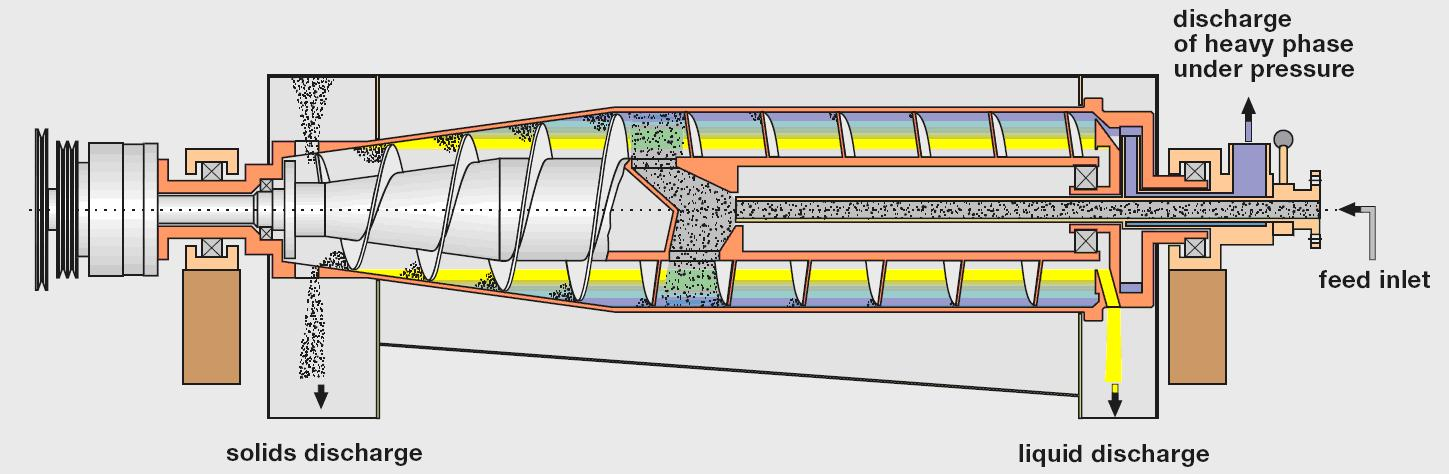
\includegraphics[width=0.8\textwidth]{images/tricanter}
	\caption{Esquema d'un tricànter}
	\label{fig:tricanter}
\end{figure}

\begin{figure}[H]
	\centering
	\animategraphics[autoplay, loop, poster =none]{20}{images/tricanter-movie/tricanter-movie-}{0}{384}
	\caption{Animació explicativa de com funciona un tricanter}
\end{figure}


Així doncs un cop descrit el sistema es poden veure els factors que s'hauran de controlar per tal de realitzar l'estudi:

\begin{itemize}
	\item Volum al dipòsit C-03 (en kg)
	\item Velocitat de la bomba P-C32 (en Hz)
	\item Cabal d'entrada al tricànter T-05
	\item Diferència de velocitats entre els cilindres interior i exterior
\end{itemize}

\end{document}